\documentclass[12pt]{article}
\usepackage[english]{babel}
\usepackage[margin=0.80in]{geometry}
\usepackage{amsmath}
\usepackage{amssymb}
\usepackage{algorithm}
\usepackage[noend]{algpseudocode}
\usepackage[utf8]{inputenc}
\usepackage{graphicx}
\usepackage{listings}
\usepackage{color}
\usepackage{hyperref}
\usepackage{cite}
%\usepackage{textcomp,uiosloforside}
\numberwithin{figure}{section}
\numberwithin{table}{section}

\definecolor{mygreen}{rgb}{0,0.6,0}
\definecolor{mymauve}{rgb}{0.58,0,0.82}
\definecolor{mygray}{rgb}{0.97,0.97,0.97}
	
\lstset{
	language=C++,
	basicstyle=\footnotesize,
	commentstyle=\color{mygreen},
	keywordstyle=\color{blue},
	stringstyle=\color{mymauve},
	tabsize=4
}

\begin{document}
\begin{titlepage}
\title{Project 2 - FYS4150}
\author{Trude Hjelmeland, Oda Langrekken and Jostein Brændshøi}
%\date{\today}
\date{%
    Department of Physics\\%
    University of Oslo\\[2ex]%
    \today
}
\clearpage
\maketitle
\thispagestyle{empty}

\begin{abstract}
\noindent We use the Jacobi eigenvalue method to solve the Schrödinger equation for an electron in a harmonic potential as well as for two interacting electrons, and thus find the energies and wavefunctions of the electrons. As we know the exact result for the former case, we find that the numerical method finds consistent eigenvalues. However we will see that the algorithm is not very efficient.
\end{abstract}
\vspace{2.00cm}

\noindent The address \url{https://github.com/jostbr/FYS4150-Projects/tree/master/Project2} on Git-Hub is associated with this project. Here one can find all code used in the project. This includes C++ source files containing the core of the project, header files, but also Python plotting scripts for result visualization. There are also available benchmark results from running the code as well as \LaTeX \ source for this PDF.

\end{titlepage}
\pagebreak

% ========
% ======== Indicate new section
% --------
% -------- Indicate new subsection
% ----- Indicate new subusub section

% ========================================================================================
% ========================================================================================
\section{Introduction}

\noindent  According to Wikipedia\cite{physics} physics  "is the natural science that involves the study of matter and its motion and behavior through space and time". In classical mechanics the motion of a system through space and time is described by its position $\vec{r}$ which can be determined by applying Newton's second law: $\vec{F}=m\vec{a}$. In quantum mechanics, the state of a system is described by its wavefunction $\Psi$, and we get it by solving the Schrödinger equation \cite{Qm}  $$-\frac{\hbar^2}{2m}\nabla^2\Psi+V\Psi=i\hbar \frac{\partial \Psi}{\partial t}$$
The Schrödinger equation can be solved analytically for a couple of simple systems, among them the hydrogen atom. For more complex systems, take the helium atom as an example, the equation is analytically unsolvable. Fortunately for us physicists, the equation can often be simplified and the solution approximated by numerical algorithms.   \\


\noindent In this project we have developed a general eigenvalue solver utilizing Jacobi's rotational algorithm to solve the Schrödinger equation for a electron in a confining potential, visualized as a quantum dot or an electron in a box with infinite walls. We will further expand our model to include the repulsive coulomb forces acting between two electrons confined in a three dimensional harmonic oscillator potential. We will show that these are essentially eigenvalue problems on a tridiagonal matrix form which we can solve numerically utilizing Jacobi's rotational algorithm.   \\

\noindent First we will examine some of the theory used in this project, most notably the solution of the Schrödinger equation and the concept of similarity transformations in linear algebra. We then move on to discuss how the Schrödinger equation can be reduced to an eigenvalue problem through discretization and how this problem can be solved by using the Jacobi method. Next we introduce some of the unit tests used to check the functionality of our program. We then present our results, both for the one-electron and the two-electron case. Finally we offer some concluding remarks about solving the Schrödinger equation numerically using the Jacobi method.

% ========================================================================================
% ========================================================================================
\section{Theory}

%-----------------------------------------------------------------------------------
%-----------------------------------------------------------------------------------
\subsection{Schrödinger equation}
\noindent The evolution of a quantum mechanical system is described by the Schrödinger equation \cite{Qm}
\begin{equation}
\label{schrodinger}
-\frac{\hbar^2}{2m}\nabla^2\Psi+V\Psi=i\hbar \frac{\partial \Psi}{\partial t}
\end{equation}
If the potential is independent of time, $V=V(\vec{r}) 
$, separation of variables lead to the time-independent Schrödinger equation  $\hat{\mathcal{H}} \psi_i = E_i \psi_i$ where $\hat{\mathcal{H}}$ is the Hamiltonian, the quantum mechanical energy operator
$$\hat{\mathcal{H}}=-\frac{\hbar^2}{2m}\nabla^2+V$$and $E_i$ is the energy of the system described by the wave function $\psi_i$. The Schrödinger equation \eqref{schrodinger} has been reduced to a eigenvalue problem, where the energy $E_i$ of a state $\psi_i$ can be found by acting on the state with the Hamiltonian. The energies $E_i$ are the eigenvalues of the Hamiltonian matrix, and the states $\psi_i$ are their corresponding eigenvectors.\\

\noindent In this project we will look at the radial part of the time-independent Schrödinger equation for an electron moving in a three-dimensional harmonic oscillator potential. Assuming spherical symmetry, the equation to be solved is \cite{pro2} 

\begin{equation}
\label{eq:radial}
  -\frac{\hbar^2}{2 m} \left ( \frac{1}{r^2} \frac{d}{dr} r^2
  \frac{d}{dr} - \frac{l (l + 1)}{r^2} \right )R(r) 
     + V(r) R(r) = E R(r).
\end{equation}



\noindent Here $E$ and $V(r)$ are the energy and potential of the harmonic oscillator respectively.\\ The potential of an harmonic oscillator is on the form $(1/2)kr^2$ with $k=m\omega^2$. Here $m$ is the electron mass, $k$ is a force constant and $\omega$ is the oscillator frequency. The energies are generally determined by \cite{pro2}

\begin{equation}
E_{nl}=  \hbar \omega \left(2n+l+\frac{3}{2}\right), \textrm{for} \hspace{0.1cm} n=0,1,2,\dots \textrm{and}  \hspace{0.1cm} l=0,1,\dots n-1
\end{equation}

\noindent but we will limit ourselves to the case where the quantum number for the orbital angular momentum of the electron is zero, specifically that $l=0$. The spherical coordinate transformation means that $r\in [0,\infty)$, and we substitute $R(r)$ in equation \eqref{eq:radial} with  $(1/r) u(r)$ where $u(r)$ is the wave function. We use the boundary conditions $u(0)=0$ and $u(\infty)=0$. The equation now reads \cite{pro2}

\begin{equation}
\label{eq:radial2}
  -\frac{\hbar^2}{2 m} \frac{d^2}{dr^2} u(r) 
       + V(r) u(r)  = E u(r) .
\end{equation}


\noindent We want to scale our equations by introducing a dimensionless variable $\rho $ instead of our position variable $r$. We do so by defining a dimensionless variable $\rho = (1/\alpha) r$, where the constant $\alpha$ has dimensions of length. Inserting this in equation \eqref{eq:radial2} gives \cite{pro2}


\begin{equation}
\label{eq:radial3}
  -\frac{\hbar^2}{2 m \alpha^2} \frac{d^2}{d\rho^2} u(\rho) 
       + V(\rho) u(\rho)  = E u(\rho) .
\end{equation}

\noindent Inserting the harmonic oscillator potential $V(\rho) = (1/2) k \alpha^2\rho^2$ we get \cite{pro2}

\begin{equation}
\label{radial4}
  -\frac{\hbar^2}{2 m \alpha^2} \frac{d^2}{d\rho^2} u(\rho) 
       + \frac{k}{2} \alpha^2\rho^2u(\rho)  = E u(\rho) .
\end{equation}
\noindent We want to simplify the equation \eqref{radial4}, and get it on the form \cite{pro2}

\begin{equation}
\label{eq:radial_num}
  -\frac{d^2}{d\rho^2} u(\rho) + \rho^2u(\rho)  = \lambda u(\rho) .
\end{equation}

\noindent We obtain equation \eqref{eq:radial_num} by first multiplying both sides of equation \eqref{radial4} with $2m\alpha^2/\hbar^2$ and defining $\lambda$ as \cite{pro2}

\begin{equation}
\lambda = \frac{2m\alpha^2}{\hbar^2}E,
\end{equation}

%In three dimensions the eigenvalues for $l=0$ are $\lambda_0=3,\lambda_1=7,\lambda_2=11,\dots .$

\noindent This allows us to fix the constant $\alpha$ so that \cite{pro2}

\begin{equation}
\alpha = \left(\frac{\hbar^2}{mk}\right)^{1/4}.
\end{equation}

\noindent We move on to the interacting case, but will come back to the above in section \ref{sec:discretization}.


%-----------------------------------------------------------------------------------
%-----------------------------------------------------------------------------------
\subsection{The two-electron Schrödinger equation}
So far our system has consisted of only one electron. If we want to study a two-electron system, the situation gets a little more complex. The two electrons will still be in a harmonic oscillator potential, but they now in addition interact with each other through Coulomb forces. If we forget about the Coulomb potential for a little while, the two-electron wave equation is \cite{Comp}
\begin{equation}
\label{two:schrodinger}
\left(-\frac{\hbar^2}{2m}\frac{d^2}{dr^2_1}-\frac{\hbar^2}{2m}\frac{d^2}{dr^2_2}+\frac{1}{2}kr^2_1+\frac{1}{2}kr^2_2\right)u(r_1,r_2)=E^{(2)}u(r_1,r_2)
\end{equation}
where $E^{(2)}=E_1+E_2$ is the energy of the two electrons. \\

\noindent We now introduce the relative coordinate $\vec{r}=\vec{r}_1-\vec{r}_2$ and the center-of-mass coordinate $R=\frac{1}{2}\left(\vec{r}_1+\vec{r}_2\right)$. The Schrödinger equation now reads
\begin{equation}
\label{schrodinger:sep}
\left(-\frac{\hbar^2}{m}\frac{d^2}{dr^2}-\frac{\hbar^2}{4m}\frac{d^2}{dR^2}+\frac{1}{4}kr^2+kR^2\right)u(r,R)=E^{(2)}u(r,R)
\end{equation}
We assume the wave function can be separated into a function of $r$ and a function of $R$, $u(r,R)=\psi(r)\phi(R)$. We are only interested in the r-dependent equation, so equation \eqref{schrodinger:sep} becomes 
\begin{equation}
\label{r:schrodinger}
\left(-\frac{\hbar^2}{m}\frac{d^2}{dr^2}+\frac{1}{4}kr^2\right)\psi(r)=E_r\psi(r)
\end{equation}
Now that we have an equation for two electrons in a harmonic oscillator potential, we can add the repulsive Coulomb potential. The Coulomb potential between an electron at position $\vec{r}_1$ and an electron at position $\vec{r}_2$ is 
$$V(\vec{r}_1,\vec{r}_2)=\frac{\beta e^2}{\vec{r}_1-\vec{r}_2}$$
where $e$ is the electron charge and $\beta$ is a constant. Using our relative coordinate $r$ , we have 
$$V(\vec{r}_1,\vec{r}_2)=\frac{\beta e^2}{r}$$
Inserting this into \eqref{r:schrodinger} we get the Schrödinger equation for two interacting electrons in a harmonic oscillator potential
\begin{equation}
\label{schrodinger:interacting}
\left(-\frac{\hbar^2}{m}\frac{d^2}{dr^2}+\frac{1}{4}kr^2+\frac{\beta e^2}{r}\right)\psi(r)=E_r\psi(r)
\end{equation}We again introduce the dimensionless variable $\rho$, and our scaled equation is
\begin{equation}
\label{schrodinger:interacting scaled}
\left(-\frac{\hbar^2}{m\alpha^2}\frac{d^2}{d\rho^2}+\frac{1}{4}k\alpha^2\rho^2+\frac{\beta e^2}{\alpha\rho}\right)\psi(\rho)=E_\rho\psi(\rho)
\end{equation}
We now define a new frequency
\begin{equation}
	\label{eq:omegar}
 \omega_r^2=\frac{1}{4}\frac{mk}{\hbar^2}\alpha^4
\end{equation}

\noindent and be requiring $m\alpha\beta e^2/\hbar^2=1$, we have 
$$\alpha = \frac{\hbar^2}{m\beta e^2}$$
By also defining
$$\lambda = \frac{m\alpha^2}{\hbar^2}E$$
our wave equation reads
\begin{equation}
\label{schrodinger:interacting final}
-\frac{d^2}{d\rho^2}\psi(\rho)+\omega^2_r\rho^2\psi(\rho)+\frac{1}{\rho}\psi(\rho)=\lambda\psi(\rho)
\end{equation}

\noindent We now move on to some linear algebra, but as with the single electron case, we will come back to the above in section \ref{sec:discretization}.

%-----------------------------------------------------------------------------------
%-----------------------------------------------------------------------------------
\subsection{Some linear algebra} \label{sec:linalg}

\noindent From linear algebra \cite{Comp} we know that if we have a real symmetric matrix, meaning that $\mathbf{A} \in \mathbb{R}^{n\times n}$, which have $n$ distinct or not eigenvalues $\lambda_1, ..., \lambda_{n} $ it is possible, through similarity transformations on the original matrix $\mathbf{A}$, to obtain the eigenvalues as the non zero elements found on the leading diagonal of a diagonal matrix $\mathbf{D}$. So if $\mathbf{A}$ is real and symmetric then a real orthogonal matrix $\mathbf{S}$ exists such that $\mathbf{S}^T \mathbf{A} \mathbf{S} = \mathbf{D}$. The statement that $\mathbf{B}$ is a similarity transform of $\mathbf{A}$ is true \cite{Comp} if $\mathbf{B} = \mathbf{S}^T \mathbf{A} \mathbf{S}$ where the condition $\mathbf{S}^T \mathbf{S} = \mathbf{S}^{-1} \mathbf{S} = \mathbf{I}$, where $\mathbf{I}$ is the identity matrix, is met. So the strategy for the upcoming algorithm will be to preform a series of similarity transforms (where each transformation moves the matrix closer to diagonal from) on matrix $\mathbf{A}$ so that

\begin{equation}
 \mathbf{S_N}^T \cdots \mathbf{S_1}^T \mathbf{A} \mathbf{S_1} \cdots \mathbf{S_N} = \mathbf{D} 
\end{equation}
and $\mathbf{D}$ then contains the eigenvalues along the diagonal. But for this to work, the eigenvalues must stay the same after a similarity transformation. \\

\noindent An important property of a similarity transformation is that the eigenvalues are conserved even though the eigenvectors are changed \cite{Comp}. To see this we look at a general eigenvalue problem on the form
\begin{equation}
	\mathbf{A} \mathbf{x}  = \lambda \mathbf{x} \label{eq:eig_og}
\end{equation}
and a similarity transformed matrix $\mathbf{B}$, more accurate that $\mathbf{B} = \mathbf{S}^T \mathbf{A} \mathbf{S}$. If we now multiply \eqref{eq:eig_og} with $\mathbf{S}^T$ from the left and insert $\mathbf{S}^{-1} \mathbf{S} = \mathbf{I}$ between $\mathbf{A}$ and $\mathbf{x}$ we have that 

\begin{equation}
	(\mathbf{S}^T \mathbf{A} \mathbf{S}) (\mathbf{S}^T \mathbf{x}) = \lambda \mathbf{S}^T \mathbf{x}
\end{equation}

\noindent which we immediately recognize is the same as 

\begin{equation}
	\mathbf{B} (\mathbf{S}^T \mathbf{x}) =  \lambda \mathbf{S}^T \mathbf{x}
\end{equation}

\noindent It is now clear to see that the eigenvalue $\lambda$ of matrix $\mathbf{A}$ is also a eigenvalue of $\mathbf{B}$ but that the eigenvector of $\mathbf{B}$ equal $\mathbf{S}^T \mathbf{x}$ is not the same as the eigenvector of $\mathbf{A}$ equal to $\mathbf{x}$. We could repeat this argument for a series of such transforms and generally we then have that the eigenvalues are preserved for an arbitrary number of such transforms. This is very important for the algorithm below to make sense and produce correct results. \\

\noindent One additional theoretical result worth visiting before talking about the algorithm, regards the fact that a similarity transformation preserves orthogonality and the dot product. In order to prove this we look at a given basis $\mathbf{v}_i\in\mathbb{R}^n$ of vectors
\begin{equation*}
    \mathbf{v}_i=
        \begin{bmatrix}
        	v_{i1} \\
            \vdots \\
            v_{in} \\
        \end{bmatrix}
\end{equation*}
and assume that the basis is orthogonal, i.e.
\begin{equation*}
	\mathbf{v}_j^T\cdot\mathbf{v}_i=\delta_{ij} \ , \qquad \delta_{ij}=
    	\begin{cases}
			1 \ , \ i=j\\
			0 \ , \ i\neq j
		\end{cases}
\end{equation*}
Then we define an orthogonal matrix $\mathbf{U}\in\mathbb{R}^{n\times n}$ in the orthogonal transformation $\mathbf{w}_i=\mathbf{U}\mathbf{v}_i$. Using matrix-vector multiplication properties, the transformed dot product evolves as
\begin{align*}
	\mathbf{w}_j^T\cdot\mathbf{w}_i&=(\mathbf{U}\mathbf{v}_j)^T\cdot (\mathbf{U}\mathbf{v}_i)=\mathbf{U}^T\mathbf{v}_j^T\cdot \mathbf{U}\mathbf{v}_i=\mathbf{U}^T\mathbf{U}\mathbf{v}_j^T\cdot\mathbf{v}_i \\
&=\mathbf{U}^{-1}\mathbf{U}\mathbf{v}_j^T\cdot\mathbf{v}_i=\mathbf{I}\mathbf{v}_j^T\cdot\mathbf{v}_i=\delta_{ij}
\end{align*}
where $\mathbf{I}\in\mathbb{R}^{n\times n}$ is the identity matrix and the third last equality holds due to $\mathbf{U}^T=\mathbf{U}^{-1}$ for orthogonal matrices. So then we see that the dot product is preserved by an orthogonal transformation. And since the dot product is preserved we note that the transformed basis $\mathbf{w}_i$ also is orthogonal and thus, the orthogonal transformation also preserves orthogonality. We now move on to look at the algorithms utilizing this result for solving the eigenvalue problem relevant for this project.

%Jeg føler at dette er nå er vist!! YEAH!!
% Enig! Ser veldig bra ut! Nice! Jeg prøver å flette det inn i jacobi seksjonen.

% ========================================================================================
% ========================================================================================
\section{Methods}
\subsection{Discretization} \label{sec:discretization}

%I did not include this intermediate step in the calculation 
%\begin{equation*}
%  -\frac{d^2}{d\rho^2} u(\rho) 
%       + \frac{mk}{\hbar^2} \alpha^4\rho^2u(\rho)  = \frac{2m\alpha^2}{\hbar^2}E u(\rho) .
%\end{equation*}

\noindent Now we want to numerically approximate equation \eqref{eq:radial_num} and recognize the first term, the second derivative, as the same we had in project 1 \cite{pro1} and recall that this can be approximated trough the three point formula \cite{Comp}

\begin{equation}
\label{eq:3point}
 \frac{d^2}{d\rho^2} u(\rho) = \frac{u(\rho+h) -2u(\rho) +u(\rho-h)}{h^2} +O(h^2)
\end{equation}

\noindent where $O(h^2)$ is the truncation error we make by terminating the Taylor expansion after only a few terms instead of including the whole series. Here h is our step size and defined by the total number of mesh points N and our choice of $\rho_0$ and $\rho_{max}$ \cite{Comp} 

\begin{equation}
\label{eq:h}
  h=\frac{\rho_{max}-\rho_0 }{N}.
\end{equation}

\noindent In our case we set $\rho_0$ equal to zero and preferably we would want $\rho_{max}$ to be $\infty$ but in our numerical approximation we need to set $\rho_{max}$ to a finite number. We discretize the rest of our $\rho$ values through $\rho_i= \rho_0 + ih$ for $i=1,2,\dots , N-1$. This discretization allows us to rewrite time-independent Schrödinger equation as \cite{pro2}

\begin{equation}
 -\frac{u(\rho_i+h) -2u(\rho_i) +u(\rho_i-h)}{h^2}+\rho_i^2u(\rho_i)  = \lambda u(\rho_i)
\end{equation}

\noindent Where $\rho_i ^2$ is the harmonic oscillator potential, $V_i$. Now we see that this essentially is a problem on a tridiagonal matrix form and define the leading diagonal elements as $d_i$ and the off diagonal elements $e_i$ through \cite{pro2}

\begin{equation*}
   d_i=\frac{2}{h^2}+V_i,
\end{equation*}

\noindent and 

\begin{equation*}
   e_i=-\frac{1}{h^2}.
\end{equation*}

\noindent Here we realize that all off-diagonal elements are equal constants further simplifying our expression for the time-independent Schrödinger equation to \cite{pro2}

\begin{equation}
d_iu_i+e_{i-1}u_{i-1}+e_{i+1}u_{i+1}  = \lambda u_i, \label{eq:discrete_eq}
\end{equation}

\noindent With $u_i$ as unknown. To further visualize that we have reduced our problem to a eigenvalue problem on a tridiagonal matrix form we write \cite{pro2}

\begin{equation}
    \begin{bmatrix}d_0 & e_0 & 0   & 0    & \dots  &0     & 0 \\
                                e_1 & d_1 & e_1 & 0    & \dots  &0     &0 \\
                                0   & e_2 & d_2 & e_2  &0       &\dots & 0\\
                                \dots  & \dots & \dots & \dots  &\dots      &\dots & \dots\\
                                0   & \dots & \dots & \dots  &\dots  e_{N-1}     &d_{N-1} & e_{N-1}\\
                                0   & \dots & \dots & \dots  &\dots       &e_{N} & d_{N}
             \end{bmatrix}  \begin{bmatrix} u_{0} \\
                                                              u_{1} \\
                                                              \dots\\ \dots\\ \dots\\
                                                              u_{N}
             \end{bmatrix}=\lambda \begin{bmatrix} u_{0} \\
                                                              u_{1} \\
                                                              \dots\\ \dots\\ \dots\\
                                                              u_{N}
             \end{bmatrix} \label{eq:eig_rep}
\end{equation}

\noindent Here it is important to note that the two end endpoints $\rho_0$ and $\rho_{max}$ are known through the boundary conditions so we omit  these values when we construct our matrix giving us the matrix \cite{pro2} 

\begin{equation}
    \begin{bmatrix} \frac{2}{h^2}+V_1 & -\frac{1}{h^2} & 0   & 0    & \dots  &0     & 0 \\
                                -\frac{1}{h^2} & \frac{2}{h^2}+V_2 & -\frac{1}{h^2} & 0    & \dots  &0     &0 \\
                                0   & -\frac{1}{h^2} & \frac{2}{h^2}+V_3 & -\frac{1}{h^2}  &0       &\dots & 0\\
                                \dots  & \dots & \dots & \dots  &\dots      &\dots & \dots\\
                                0   & \dots & \dots & \dots  &-\frac{1}{h^2}  &\frac{2}{h^2}+V_{N-2} & -\frac{1}{h^2}\\
                                0   & \dots & \dots & \dots  &\dots       &-\frac{1}{h^2} & \frac{2}{h^2}+V_{N-1}
             \end{bmatrix} \label{eq:relevantA}
\end{equation}

\noindent where $V_i=\rho_i^2$. \\

\noindent The two-electron wave equation \eqref{schrodinger:interacting final} can be discretized in much the same way. The expressions for the diagonal and off-diagonal matrix elements still hold, but the potential is now given by
$$V_i=\omega_r^2\rho_i^2+\frac{1}{\rho_i}$$


%-----------------------------------------------------------------------------------
%-----------------------------------------------------------------------------------
\subsection{Jacobi rotation algorithm}
Now that we have arrived at the final discretized formulation \eqref{eq:discrete_eq} of the differential equation \eqref{eq:radial_num} we can look in to methods for solving the equation. As stated before, we are dealing with an eigenvalue problem illustrated by \eqref{eq:eig_rep} with the matrix given by \eqref{eq:relevantA}. Thus we want to implement a numerical method for solving for eigenvalues and eigenvectors in order to obtain the wavefunction for the different energies. In particular we will discuss and implement the Jacobi rotation algorithm. This algorithm is designed for dense symmetric matrices (which is the case for us) and is based on performing a series of orthogonal transformations in order to get the matrix in question on diagonal form (as discussed in section \ref{sec:linalg}). Orthogonal transformations require an orthogonal matrix $\mathbf{S}$ and, for the Jacobi algorithm, this matrix is a classical rotation matrix generalized for higher dimensions. That is
\begin{equation}
	\mathbf{S} = \begin{bmatrix}
                           1& \cdots & 0 & \cdots  & 0 & \cdots & 0 \\
                           \vdots & \ddots & \vdots &  & \vdots & & \vdots \\
                           0 &  & \cos(\theta) & \cdots & -\sin(\theta) & \cdots & 0 \\
                           \vdots & & \vdots & \ddots & \vdots & & \vdots \\
                           0 &  & \sin(\theta) & \cdots & \cos(\theta) & \cdots & 0 \\
                           \vdots & & \vdots & & \vdots & \ddots & \vdots \\
                           0 & \cdots & 0 & \cdots  & 0 & \cdots & 1
                      \end{bmatrix} \label{matrixA}
\end{equation}
Then, a single orthogonal transformation $\mathbf{A}'$ of $\mathbf{A}$ can be written as
\begin{equation}
	\mathbf{A}'=\mathbf{S}^T\mathbf{A}\mathbf{S} \label{eq:orth_transf}
\end{equation}
And since $\mathbf{S}$ is orthogonal, this transformation corresponds to the similarity transformation $\mathbf{A}'=\mathbf{S}^{-1}\mathbf{A}\mathbf{S}$. Also, due to the sparse form of $\mathbf{S}$, the double matrix product in \eqref{eq:orth_transf} results in only a few elements $a_{ij}$ of $\mathbf{A}$ being affected. Assume that the upper and lower "trigonometric row" in $\mathbf{S}$ are located at index $k$ and $l$, respectively. Such a rotation "sub matrix" is also square implying that column-wise the indices are $k$ and $l$ as well ($k<l$). Also let $i\in[1,2,...,n]$ where $n\times n$ is the size of the matrix. Then when performing the product \eqref{eq:orth_transf} only the following elements of $\mathbf{A}$ are affected \cite{Comp}:
\begin{align}
	a_{ii}'&=a_{ii} \ , \qquad i\neq k, \ i\neq l \nonumber \\
    a_{ik}'&=a_{ik}\cos(\theta)-a_{il}\sin(\theta) \ , \qquad i\neq k, \ i\neq l \nonumber  \\
    a_{il}'&=a_{il}\cos(\theta)+a_{ik}\sin(\theta) \ , \qquad i\neq k, \ i\neq l \nonumber  \\
    a_{kk}'&=a_{kk}\cos^2(\theta)-2_a{kl}\cos(\theta)\sin(\theta)+a_{ll}\sin^2(\theta) \label{eq:bikl}\\
    a_{ll}'&=a_{ll}\cos^2(\theta)+2a_{kl}\cos(\theta)\sin(\theta)+a_{kk}\sin^2(\theta) \nonumber \\
    a_{kl}'&=(a_{kk}-a_{ll})\cos(\theta)\sin(\theta)+a_{kl}\left[\cos^2(\theta)-\sin^2(\theta)\right] \nonumber 
\end{align}
The fact that only these elements are affected can be visualized easier by for example doing this transformation by hand for a $3\times 3$ matrix. We see that generally one such transformation does not form a diagonal matrix as only some elements in the matrix change. Although, the idea performing such a transformation many times while changing $k$ and $l$ for each transformation, seems reasonable. Also, while performing many such transformations, eventually leading to a diagonal matrix, we know, from the linear algebra \cite{LinAlg}, that the "total" transformation matrix converting $\mathbf{A}$ to diagonal form, contains the eigenvectors of $\mathbf{A}$ as columns. In our case this total transformation matrix is the product of all the $\mathbf{S}$ matrices we compute for each transformation, i.e. $\mathbf{V}=\mathbf{S}_1\mathbf{S}_2\cdots\mathbf{S_m}$ (if $m$ iterations produces the diagonal matrix). Using this we can update the eigenvectors for each transformation \cite{Comp}
\begin{align}
	v_{ik}'=v_{ik}\cos(\theta)-v_{il}\sin(\theta) \label{eq:eigvec_1}\\
    v_{il}'=v_{il}\cos(\theta)+v_{ik}\sin(\theta) \label{eq:eigvec_2}
\end{align}
Again, the reason for these simple expressions is that $\mathbf{S}(k,l,\theta)$ is quite sparse in its form and thus only affects a few elements when updating the eigenvectors. Even though this looks like a decent start, we don't yet know the values of $\cos(\theta)$ and $\sin(\theta)$. Let's look into this issue. \\

\noindent We wish to obtain a diagonal matrix through a series transformations (such as \eqref{eq:bikl} and thus would like to require the non-diagonal elements to be zero. Here this corresponds to $a_{kl}'=0$ (the lower equation in \eqref{eq:bikl}). We would like to set this to zero for every such transformation and reasonable choices for $k$ and $l$ are discussed below. Requiring $a_{kl}'=0$ puts a constraint on $\cos(\theta)$ and $\sin(\theta)$. In particular, if $a_{kl}=0$ as well, we see that $\cos(\theta)=1$ and $\sin(\theta)=0$. If $a_{kl}\neq 0$ we can divide by $\cos^2(\theta)$ and recognize $\tan(\theta)=\sin(\theta)/\cos(\theta)$ to get
\begin{equation}
	\frac{a_{kk}-a_{ll}}{a_{kl}}\tan(\theta)-\tan^2(\theta)+1=0 \qquad\Rightarrow\qquad \tan^2(\theta)+2\tau\tan(\theta)-1=0 \label{eq:tan_zero}
\end{equation}
with $\tau=(a_{ll}-a_{kk})/2a_{kl}$. This is a quadratic equation for $\tan(\theta)$ and has solutions
\begin{equation}
	\tan(\theta)=-\tau\pm\sqrt{1+\tau^2}
\end{equation}
and further yields
\begin{equation}
	\cos(\theta)=\frac{1}{\sqrt{1+\tan^2(\theta)}} \ , \qquad \sin(\theta)=\cos(\theta)\tan(\theta)
\end{equation}
through trigonometric identities. Having obtained the values for $\cos(\theta)$ and $\sin(\theta)$ allows us to calculate the elements of the transformed matrix through \eqref{eq:bikl} and update the eigenvectors through \eqref{eq:eigvec_1} and \eqref{eq:eigvec_2}. The only remaining question now is how to choose $k$ and $l$ for each transformation. Letting $k$ and $l$ be the indices of the largest non-diagonal element in $\mathbf{A}$, i.e.
\begin{equation}
	a_{kl}=\max_{i\neq j}a_{ij}
\end{equation}
seems reasonable because then, for every transformation, we force the largest non-diagonal element of $\mathbf{A}$
to be zero through \eqref{eq:tan_zero}. This choice of $k$ and $l$ gives the largest shift towards a diagonal matrix for every transformation. \\

\noindent The above was an attempt at describing the functionality of the algorithm, but now it's time to look at the actual algorithm that we have implemented. See algorithm \ref{alg:jacobi}. Our implementation follows the basic ideas presented in algorithm \ref{alg:jacobi}, but the structure of the code is not identical to that of the algorithm. This is due to a lot of other code technical issues that need to be taken care of.

\begin{algorithm}
\caption{Jacobi algorithm} \label{alg:jacobi}
\begin{algorithmic}[1]
\Procedure{jacobi\_eigen}{$A,N$}
	\While {max\_non\_diag $>$ tolerance}
      \State \textit{// Find max non-diagonal element} \\
      \For {$i=0$ to $i=N-2$}
          \For {$j=i+1$ to $i=N-1$}
              \If {abs$(a_{ij})>$ max\_non\_diag}
                  \State max\_non\_diag = abs$(a_{ij})$
                  \State $k=i$
                  \State $l=j$
              \EndIf
          \EndFor
      \EndFor \\

      \State \textit{// Find cosine, sine values for transformation matrix}
      \If {$a_{kl} \neq 0$}
          \State $\tau = (a_{ll} - a_{kk})/2a_{kl}$
          \State $\tan(\theta) = -\tau - \sqrt{1 + \tau^2}$ \ \ \ \ \ \ \textit{// Choose smallest}
          \State $\cos(\theta) = 1/\sqrt{1 + \tan(\theta)^2}$ \ \ \ \ \textit{// Trig identity for cosine}
          \State $\sin(\theta) = \tan(\theta)*\cos(\theta)$ \ \ \ \ \ \ \textit{// Trig identity for sine}
      \Else
          \State $\cos(\theta) = 1$
          \State $\sin(\theta) = 0$
      \EndIf \\

      \State \textit{// Loop over diagonal}
      \For {$i=0$ to $i=N-1$} \\
      	  \State \textit{// Execute transformation $A'=S^TAS$}
          \If {$i \neq k$ \textbf{and} $i\neq l$}
              \State $a_{ii}'=a_{ii}$
              \State $a_{ik}'=a_{ik}\cos(\theta)-a_{il}\sin(\theta)$
              \State $a_{il}'=a_{il}\cos(\theta)+a_{ik}\sin(\theta)$
          \EndIf \\

          \State $v_{ik}' = v_{ik}\cos(\theta) - v_{il}\cos(\theta)$ \ \ \textit{// Update eigenvector component}
          \State $v_{il}' = v_{il}\cos(\theta) + v_{ik}\sin(\theta)$ \ \ \ \textit{// Update eigenvector component}

      \EndFor \\

      \State $a_{kk}'=a_{kk}\cos^2(\theta)-2a_{kl}\cos(\theta)\sin(\theta)+a_{ll}\sin^2(\theta)$
      \State $a_{ll}'=a_{ll}\cos^2(\theta)+2a_{kl}\cos(\theta)\sin(\theta)+a_{kk}\sin^2(\theta)$
      \State $a_{kl}=0$ \qquad\qquad\qquad \textit{// Force max-non diag to be zero}
      \State $a_{lk}=0$ \qquad\qquad\qquad \textit{// Force max-non diag to be zero}
    \EndWhile
    \State \Return($A, V$) \qquad \textit{// Return eigenvalues and eigenvector}
\EndProcedure
\end{algorithmic}
\end{algorithm}

\pagebreak



%-----------------------------------------------------------------------------------
%-----------------------------------------------------------------------------------
\subsection{Testing}
\label{sec:testing}
When writing code and developing software in general one often writes some functionality and then later update or make enhancments to that piece of code. Then it's easy to make changes that suddenly results in that particular code not working as it should anymore, but having the effect of the entire program producing unwanted behaviour. As a programmer, it's then often not trivial to pinpoint where in the code the source of error is. This is one area where unit tests become useful. Constructing tests for various parts of the program will help the programmer quickly localize the faulty logic and thus save time. In addition, unit tests acts as a great way to make sure some code snippet being worked on, functions as expected before movin on to write other parts of the program. Also they act as additional documentation for the code by exemplifying functionality. For computer science in general these unit tests could be testing arbitrary functionality. However in our contex, it's particularly useful for testing mathematical properties, which is the focus below. For this project we have implemented four unit tests.

%------------------------------------------------------------
\subsubsection{Max non-diagonal element test}

\noindent We have constructed a unit test to ensure that our function that finds the element with the highest absolute value of a matrix actually returns the element with the highest absolute value. We have done this by constructing a small matrix with a known maximum element and perform a function call to our function that find the maximum element. We then preform an if test to see if the maximum value actually was returned by our function. If the function finds the right element a message is prompt in the terminal window telling us that the maximum value test is passed.

%Trude skriver også om max unit test
%------------------------------------------------------------
\subsubsection{Eigenvalue test}
We also constructed a unit test to check if we have implemented the Jaocbi algorithm correctly in our program. We defined a 4x4 matrix and used Matlab to find the eigenvalues of the matrix. We then preform a function call to our Jacobi solver which returns the eigenvalues and eigenvectors. An if test checks if the correct eigenvalues are returned within a reasonable level of accuracy, $10^{-5}$, then a message is prompt in the terminal window telling the user whether the eigenvalue test is passed or not.

%------------------------------------------------------------
\subsubsection{Orthogonality test}
Another thing we wanted to test is if our implementation of algorithm \ref{alg:jacobi} preserves orthogonality as discussed in section \ref{sec:linalg}. In light of this we made a unit test using a known $5\times 5$ matrix and starting with an identity matrix $\mathbf{I}$ as a basis. Then calling on \texttt{jacobi\_eigen()} we get back the resulting eigenvectors as columns in a matrix $\mathbf{V}$. To check for orthogonality of the columns of $\mathbf{V}$ we loop through every possible combination of columns of $\mathbf{V}$ and compute the inner product of each combination. This can be done as illustrated in the code snippet below: \\

\begin{lstlisting}[backgroundcolor=\color{mygray}, frame=single, showstringspaces=false, xleftmargin=\parindent, xrightmargin=\parindent]
	for (int c_1 = 0; c_1 < N; c_1++)      // Loop through cols in V.
        for (int c_2 = 0; c_2 < N; c_2++)  // Loop through cols in V per col
            inner_prod = 0.0;

            for (int k = 0; k < N; k++)
                inner_prod += V(k,c_1)*V(k,c_2);    // Compute inner product
\end{lstlisting}

\noindent For the orthgogonality to be preserved we would need
\begin{equation}
	\mathbf{v}_{i}\cdot\mathbf{v}_j=
	\begin{cases}
			1 \ , \ i=j\\
			0 \ , \ i\neq j
		\end{cases}
\end{equation}
where $i$ and $j$ correpond respectively to column $i$ (\texttt{c\_1}) and $j$ ((\texttt{c\_2}) in $\mathbf{V}$. And indeed while running the test we observe that our implementation preserves orthogonality.

%------------------------------------------------------------
\subsubsection{Transformation matrix test}
Finally we also implemented a unit test for checking that our program finds the correct transformation mastrix, i.e. computes the correct $\cos(\theta)$ and $\sin(\theta)$ values. As with the above tests we used a known small matrix where we hand computed the $\cos(\theta)$ and $\sin(\theta)$ values and then compared the values produced by the code.

% ========================================================================================
% ========================================================================================



\section{Results}
%\noindent Some result introduction about what we have done\\

%-----------------------------------------------------------------------------------
%-----------------------------------------------------------------------------------

\noindent We want to investigate how the resulting three lowest lying eigenvalues behave as a function of the matrix size, $n$. For the non interacting case we have analytical answers for the eigenvalues and know that the three lowest eigenvalues, namely $\lambda_1$, $\lambda_2$ and $\lambda_3$, should be equal to 3, 7 and 11 respectively \cite{pro2}. Our results are enclosed in table \ref{tab:convergence} where we have used $\rho_{max} = 4.0$ and that our tolerance is $\epsilon = 10.0^{-9}$ for when the off diagonal elements are essentially zero. We have found that our solution is sensitive to choices of $\rho_{max}$ and through trial and error found that $\rho_{max} = 4.0$ is a good choice for us. \\

\noindent From table \ref{tab:convergence} we see that the eigenvalues generally get closer to the exact eigenvalues as we increase the matrix size. When we discretized the Schrödinger equation, we chose to neglect terms of order $h^2$. As $h$ is inversely proportional to the matrix size $n$ through $h = \frac{\rho_{max}-\rho_0}{n+1}$ we expect the error to decrease as we increase the matrix size. The lowest eigenvalue converges beautifully as the matrix size increases. The second and third eigenvalues seem to converge to a value a little higher than their excact value. This is probably related to our choice of $\rho_{max}$, but since the values are reasonably close to the exact values we chose not to experiment further with values for $\rho_{max}$.   \\ 


\begin{table}[h]
\begin{center}
  \begin{tabular}{| l | l | l | l |}
  \hline
    Matrix size, $n$ &  $\lambda_1$ & $\lambda_2$ & $\lambda_3$ \\[0.10cm] \hline
     5 & $2.8530$ & $6.2118$ & $9.0339$\\[0.10cm]
    10 & $2.9581$ & $6.7896$& $10.5214$\\[0.10cm]
    20 & $2.9886$& $6.9461$& $10.9307$\\[0.10cm]
    50 & $2.9981$& $6.9937$& $11.0540$\\[0.10cm]
    100 & $2.9995$& $7.0009$& $11.0725$\\[0.10cm]
    150 & $2.9998$& $7.0023$& $11.0760$\\[0.10cm]
    200 & $2.9999$& $7.0028$& $11.0772$\\[0.10cm]
    300 & $3.0000$ & $7.0031$& $11.0781$\\[0.10cm]
    400 & $3.0000$ & $7.0032$& $11.0784$\\[0.10cm]
    500 & $3.0000$ & $7.0033$& $11.0786$\\[0.10cm]
     \hline
  \end{tabular}
\end{center}
\caption{A table showing the convergence rate for the non interacting case of the three lowest eigenvalues, $\lambda_i$, as function of the matrix size, n.}
\label{tab:convergence}
\end{table}  

\begin{figure}[ht]
	\centerline{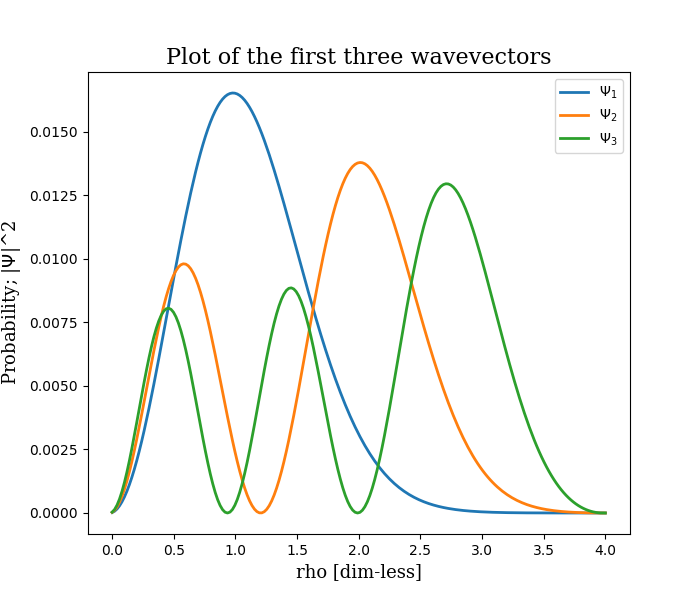
\includegraphics[scale = 0.9]{wavefunc_nonint.png}}
	\caption{Plot of the wavefunctions squared, $\psi^2$, corresponding to the three lowest eigenvalues , $\lambda_1=3, \lambda_2=7$ and $\lambda_3=11$ of an electron in a harmonic potential.}
    \label{fig:non}
\end{figure}

\noindent With two electron confined in a harmonic oscillator potential repulsive Coulomb forces acting between the two bodies are included. We have used four different oscillator frequencies, $\omega_r$, namely 0.01, 0.5, 1.0 and 5.0. The resulting wave vectors are shown in figure \ref{fig:interacting} for the three lowest lying energy states for different oscillator frequencies, $\omega_r$. \\  

%\noindent From equation \ref{eq:omegar} it is clear to see that the oscillator frequency ,$\omega_r$, scales with $\alpha$ 

\noindent We have found that our solution is sensitive to the our choice of $\rho_{max}$ for both the interacting and non interacting case. In both instances the wave function for the different energy levels should all converge towards zero in both tails. So if we chose a big $\rho_{max}$, we will include many data points of little interest where the wave function is $\sim 0$. If we look at equation \eqref{eq:h} we see how our choice of $\rho_{max}$ dictates together with the matrix size, n, our step size h. So a choice of a too large $\rho_{max}$ will lead us to loose valuable information in the regions where the wavefunctions is not equal to zero. On the other hand, choosing $\rho_{max}$ too small will make us lose part of the wavefunction. Figure \ref{fig:interacting} clearly shows why $\rho_{max}=4.0$ was such a good choice for the non-interacting case. All three wavefunctions are essentially zero above this value, and we thus include all the interesting parts of the wavefunctions in our computation. And since we do not include uninteresting regions where the wavefunctions are zero, we ensure that our step size $h$ is as small as possible while still including all regions of interest. \\

\noindent From figure \ref{fig:interacting} we see that for smaller values of $\omega_r$ a larger value of $\rho_{max}$ is needed to include all areas of interest, while when $\omega_r$ is increasing the electrons are confined to a smaller area and a smaller $\rho_{max}$ is needed. It is physically meaningful that when the oscillating potential is increasing, the repulsive energy acting between the two electrons play a less significant role and the electrons are confined in a smaller area, while when $\omega_r$ is increasing the Coulomb interaction forces the electrons to favor positions far away from each other.  \\

\noindent If we compare the plot for the one electron \ref{fig:non} with the two electron \ref{fig:interacting} situation we see that when repulsive forces are included, the wavefunctions gets stretched over a larger interval of $\rho$ for $\omega_r$ larger then 1.0. \\


\begin{figure}[ht]
	\centerline{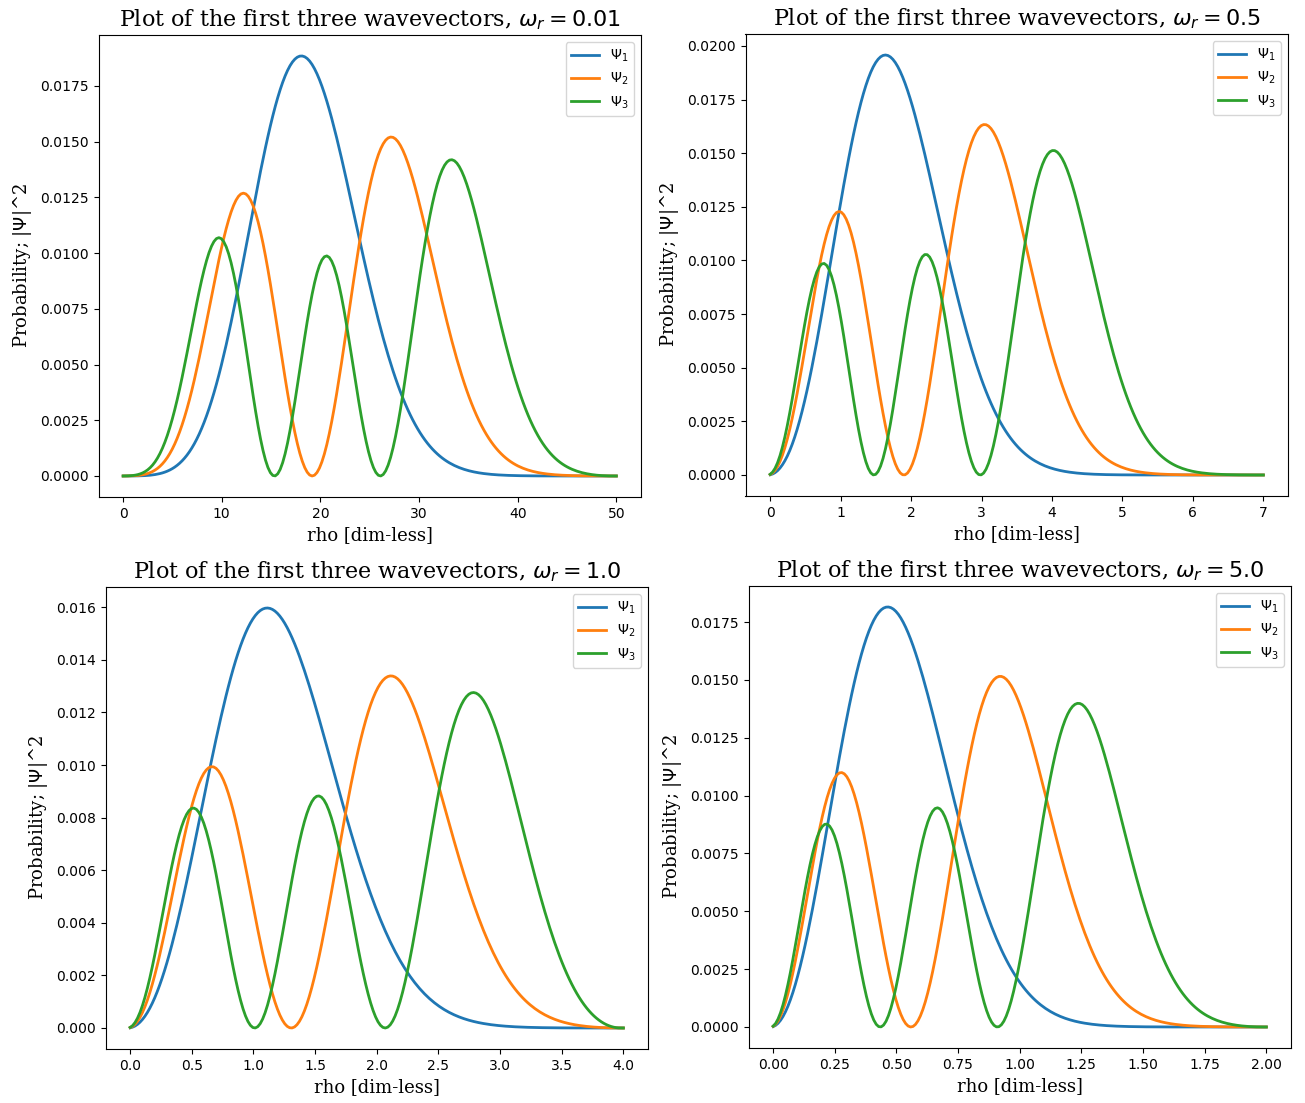
\includegraphics[scale = 0.52]{interacting_combined.png}}
	\caption{Plots of the wavefunctions squared, $\psi^2$, corresponding to the three lowest eigenvalues of two interacting electrons in a harmonic potential of frequency $\omega_r$. }
    \label{fig:interacting}
\end{figure}

\noindent It is interesting to note that our wavefunctions are orthonormal meaning that they are both orthogonal and normalized. We start our Jacobi algorithm with a identity matrix as the matrix in which the eigenvectors are to be contained. This matrix is orthonormal and the norm is conserved through our similarity transformations because the similarity transformation matrix is orthogonal \cite{LinAlg}. \\ 

\noindent Further we want to investigate how many similarity transformations are needed before all the off diagonal matrix elements are essentially equal to zero, and the matrix is diagonal. The results are enclosed in table \ref{tab:iterations}. We see that our algorithm converges towards $\sim 1.7 n^2$ similarity transformations needed already for $n = 50$. From our lecture notes \cite{Comp} we know that the number of similarity transforms needed to diagonalize a symmetric matrix is estimated to be between $3 n^2$ and $5 n^2$. Our program does not completely diagonalize the matrix, but terminates when the absolute value of the largest off-diagonal matrix elements is smaller than a certain tolerance, in our case $10.0^{-9}$. A plausible explanation for our algorithm utilizing fewer transformations that listed in our lecture notes \cite{Comp} is our choice of $\epsilon$. If we run the algorithm for $n = 200$ and use $\epsilon = 10^{-20}$, 86 087 similarity transformations are needed, resulting in a behavior of $\sim 2.2 n^2$. Where we to choose an infinitively small tolerance $\epsilon$ we would probably need between $3n^2$ and $5n^2$ transformations. Table \ref{tab:convergence} does however show that our eigenvalues are reasonably good for $\epsilon=10.0^{-9}$ transformations, and since this tolerance nearly halves the expected number of needed transformations, we see that there is a lot of time to be saved by choosing our tolerance wisely. \\



\begin{table}[h]
\begin{center}
  \begin{tabular}{| l | l | l |}
  \hline
    Matrix size, $n$ &  Number of iterations & Iterations/$n^2$ \\[0.10cm] \hline
     5 & $28$ & $1.12$ \\[0.10cm]
    10 & $148$ & $1.48$ \\[0.10cm]
    20 & $629$& $1.57$ \\[0.10cm]
    50 & $4 \hspace{0.1cm} 234$& $1.69$ \\[0.10cm]
    100 & $17 \hspace{0.1cm} 279$& $1.73$ \\[0.10cm]
    150 & $39 \hspace{0.1cm} 013$& $1.73$ \\[0.10cm]
    200 & $69 \hspace{0.1cm} 626$ & $1.74$ \\[0.10cm]
    300 & $157 \hspace{0.1cm} 213$ & $1.75$ \\[0.10cm]
    400 & $280 \hspace{0.1cm} 178$ & $1.75$ \\[0.10cm]
    500 & $439 \hspace{0.1cm} 315$ & $1.76$ \\[0.10cm]
     \hline
  \end{tabular}
\end{center}
\caption{A table showing the number of transformations needed to diagonalize a matrix of size n. We have terminated the transformations when the square of the off-diagonal matrix elements are smaller than $10.0^{-9}$ }
\label{tab:iterations}
\end{table}





\noindent How efficient is algorithm \ref{alg:jacobi}? As it turns out, not very efficient. To answer this question in more detail, lets consider a short analysis of the cost of the algorithm. When searching for the largest non-diagonal element, we utilised the fact that we have a symmetric matrix ($n\times n$). In particular this means we only need to search through the upper triangular part of the matrix, giving $0.5n^2-n$ steps (subtracting $n$ due to main diagonal not being part of search). Computing $\cos(\theta)$ and $\sin(\theta)$ only requires a couple of steps so it doesn't contribute significantly. Then performing the transformation requires $4n$ steps (neglecting what happens outside the loop). Now, all of the above happens each iteration, and, as we see from table \ref{tab:iterations}, we need $\sim 1.75n^2$ iterations before satisfactory convergence. Combining these results give a total cost of
\begin{equation}
	\text{COST}=1.75n^2(0.5n^2-n+4n)=1.75n^2(0.5n^2+3n)=0.875n^4+5.25n^3=\mathcal{O}(n^4)
\end{equation}
where the last equality illustrates the asymptotic cost of the algorithm, that is, when $n\to\infty$. So we note that the algorithm is not very efficient and this we got to experience personally when working on the project. Attempting to run the algorithm for large matrices had the potential to make us impatient at times. It's worth noting that the above used factor of 1.75 is dependent of what we choose as the tolerance for the max value (in algorithm \ref{alg:jacobi}) of the non-diagonal elements. In this case we used a tolerance of $10^{-9}$. \\

\noindent As mentioned earlier the Jacobi rotational algorithm is not the most efficient way of finding eigenvalues and eigenvectors, especially for large matrices. To clarify this point we have compared our code to Armadillos \cite{Arma} eigenvalue solver eig\_sym(). Here we have found that our eigenvalues and eigenvector are in good correlation with those found by Armadillo, but the time used differs significantly, see table \ref{tab:time}. As Armadillo uses far less time, it is obvious that there are more efficient ways of solving an eigenvalue problem numerically. \\


\begin{table}[h]
\begin{center}
  \begin{tabular}{| l | l | l |}
  \hline
    Matrix size, $n$ & Armadillo time [s] & Jacobi time [s] \\[0.10cm] \hline
    10 & $1.13\times 10^{-4}$ & $2.5\times 10^{-4}$ \\[0.10cm]
    100 & $3.03\times 10^{-3}$ & $1.39$ \\[0.10cm]
    200 & $1.48\times 10^{-2}$ & $21.99$ \\[0.10cm]
    300 & $4.13\times 10^{-2}$ & $113.96$ \\[0.10cm]
    \hline
  \end{tabular}
\end{center}
\caption{A table showing the time used by our Jacobi rotational algorithm and Armadillos function eig\_sym() as function of the matrix size, n, for the non interacting case.}
\label{tab:time}
\end{table}

%====================================================================================
%====================================================================================
\section{Concluding remarks}
\noindent For many physics students, the Schrödinger equation is part of their first introduction to quantum mechanics. Throughout a quantum mechanics course, the student will most likely solve the Schrödinger equation analytically quite a few times. The student will, however, soon realize that finding an exact solution for the energies and wavefunctions is exclusive to a couple of simple cases. As soon as more complicated potentials are introduced, i.e. two interacting electrons in a harmonic potential, the Schrödinger equation is unsolvable. Fortunately the time-independent Schrödinger equation can be reduced to an eigenvalue problem, which can be solved numerically.\\

\noindent In this project we wanted to familiarize ourselves with one of these methods, namely the Jacobi method. As we solved the Schrödinger equation for a potential where the exact solution for the energies is known, we were able to compare our results to the exact ones. Table \ref{tab:convergence} clearly shows how the solutions obtained by using the Jacobi method quickly converges towards the exact solutions, even for matrices as small as 100x100. This is fortunate, as the method is very slow for larger matrices (see table \ref{tab:time}) as uses more than a minute for matrices of size 300x300. If efficiency is not important or if we want to find the eigenvalues and eigenvectors of a small matrix, the method is an excellent choice. \\

If one were to work further on this project, it might be worthwhile to look into other more time efficient methods. In this case the matrix is tridiagonal, so a lot of time could be spared by using i.e. the bisection method to compute the eigenvalues.\\

\noindent \textbf{Personal notes:}\\
All in all we were positively surprised by the precision of the Jacobi method. When solving equations numerically one often have to choose between numerical precision and time efficiency, and if time is not an issue this is a perfect solver of eigenvalue problems. In this project we were also introduced to working with unit tests (see section \ref{sec:testing}), and we felt it really helped during development of the code. For instance, the unit test that checks if the max non-diagional element was found, saved one of us a lot of time by making us realize that our function did not work when the largest element (in absolute value) was negative.

%We can mention that our eigenvectors are orthogonormale

\pagebreak
%====================================================================================
%====================================================================================


\bibliography{sample}{}
\bibliographystyle{plain}

\end{document}